\documentclass{article}
\usepackage[accepted]{icml2018}
 % If your paper is accepted, change the options for the package
% aistats2018 as follows:
%
%\usepackage[accepted]{aistats2018}
%
% This option will print headings for the title of your paper and
% headings for the authors names, plus a copyright note at the end of
% the first column of the first page.

\usepackage{amsfonts}
\usepackage{amssymb}
\usepackage{amsmath}
\usepackage{amsthm}

\usepackage{bm}
\usepackage{cancel}
\usepackage{bbold}
\usepackage{bm}
\usepackage{slashed}
\usepackage{graphicx}
\usepackage{color}
\usepackage{algorithm}
\usepackage{algpseudocode}
\usepackage{tikz}
\usepackage{hyperref}

% Attempt to make hyperref and algorithmic work together better:
\newcommand{\theHalgorithm}{\arabic{algorithm}}

\newcommand{\glnote}[1]{\textcolor{red}{[GL: #1]}}
\newcommand{\kcnote}[1]{\textcolor{red}{[KC: #1]}}

\newcommand{\qxpsi}{q(\mathbf{x}|\bfpsi)}
\newcommand{\bftheta}{{\bm \theta}}
\newcommand{\bfpsi}{{\bm \psi}}
\newcommand{\bfphi}{{\bm \phi}}
\newcommand{\bflambda}{{\bm \lambda}}
\newcommand{\bfx}{\mathbf{x}}
\newcommand{\bfz}{\mathbf{z}}

\theoremstyle{plain}
\newtheorem{theorem}{Theorem}
\newtheorem{proposition}[theorem]{Proposition}

\icmltitlerunning{Adversarial Variational Optimization of Non-Differentiable Simulators}

\begin{document}

% If your paper is accepted and the title of your paper is very long,
% the style will print as headings an error message. Use the following
% command to supply a shorter title of your paper so that it can be
% used as headings.
%
%\runningtitle{I use this title instead because the last one was very long}

% If your paper is accepted and the number of authors is large, the
% style will print as headings an error message. Use the following
% command to supply a shorter version of the authors names so that
% they can be used as headings (for example, use only the surnames)
%
%\runningauthor{Surname 1, Surname 2, Surname 3, ...., Surname n}

\twocolumn[

\icmltitle{Adversarial Variational Optimization of\\
           Non-Differentiable Simulators}

\begin{icmlauthorlist}
\icmlauthor{Gilles Louppe}{uliege}
\icmlauthor{Kyle Cranmer}{nyu}
\end{icmlauthorlist}

\icmlaffiliation{uliege}{University of Li{\`e}ge, Belgium}
\icmlaffiliation{nyu}{New York University, USA}

\icmlcorrespondingauthor{Gilles Louppe}{g.louppe@uliege.be}
\icmlcorrespondingauthor{Kyle Cranmer}{kyle.cranmer@nyu.edu}

% You may provide any keywords that you
% find helpful for describing your paper; these are used to populate
% the "keywords" metadata in the PDF but will not be shown in the document
\icmlkeywords{XXXXX}

\vskip 0.3in
]

\printAffiliationsAndNotice{\icmlEqualContribution}


\begin{abstract}
    Complex computer simulators are increasingly used across fields
of science as generative models tying parameters of an underlying theory to
experimental observations. Inference in this setup is often difficult, as
simulators rarely admit a tractable density or likelihood function. We introduce
Adversarial Variational Optimization (AVO), a likelihood-free inference
algorithm for fitting a non-differentiable generative model incorporating ideas
from generative adversarial networks (GANs) and variational optimization. We adapt the
training procedure of Wasserstein GANs by replacing the
differentiable generative network with a domain-specific simulator. We solve the
resulting non-differentiable minimax problem by minimizing variational upper
bounds of the two adversarial objectives.
Effectively, the procedure results in
learning a proposal distribution over simulator parameters, such that
the Wasserstein distance between the marginal distribution of the synthetic data and
the empirical distribution of observed data is minimized.
We present results of the method with simulators producing both
discrete and continuous data.
\end{abstract}


% ==============================================================================

\section{Introduction}

In many fields of science such as particle physics, epidemiology  or
population genetics, computer simulators are used to describe complex data
generation processes. These simulators relate observations $\bfx$ to the
parameters $\bftheta$ of an underlying theory or mechanistic model. In most
cases, these simulators are specified as procedural implementations of forward,
stochastic processes involving latent variables $\bfz$. Rarely do these
simulators admit a tractable density (or likelihood) $p(\bfx | \bftheta)$. The
prevalence and significance of this problem has motivated an active research
effort in so-called \textit{likelihood-free inference} algorithms such as
Approximate Bayesian Computation (ABC) and density estimation-by-comparison
algorithms~\cite{beaumont2002approximate, marjoram2003markov,
sisson2007sequential, sisson2011likelihood, marin2012approximate,
cranmer2015approximating}.

In parallel, with the introduction of variational
auto-encoders~\cite{DBLP:journals/corr/KingmaW13} and generative adversarial
networks~\cite{goodfellow2014generative}, there has been a vibrant research
program around implicit generative models based on neural
networks~\cite{2016arXiv161003483M}.  While some of these models
also do not admit a tractable density, they are all differentiable by construction.
In addition, generative models based on neural networks are highly parametrized and the model
parameters have no obvious interpretation. In contrast, scientific simulators
can be thought of as highly regularized generative models as they typically have
relatively few parameters and they are endowed with some level of
interpretation. In this setting, inference on the model parameters $\bftheta$ is
often of more interest than the latent variables $\bfz$.

In this work, we develop a likelihood-free inference algorithm
for non-differentiable, implicit generative models.
We adapt the adversarial
training procedure of generative adversarial
networks~\cite{goodfellow2014generative} by replacing the implicit generative
network with a domain-based scientific simulator, and solve the resulting
non-differentiable minimax problem by minimizing variational upper
bounds~\cite{2011arXiv1106.4487W,2012arXiv1212.4507S} of the adversarial
objectives.
The objective of the algorithm is to match the marginal distribution of
the generated data to the empirical distribution of the observations.


% ==============================================================================

\section{Problem statement}
\label{sec:problem}

We consider a family of parametrized densities $p(\mathbf{x}|\bftheta)$
defined implicitly through the simulation of a stochastic generative process,
where $\mathbf{x} \in \mathbb{R}^d$ is the data and $\bftheta$ are the
parameters of interest. The simulation may involve some complicated latent
process
where $\bfz \in {\cal Z}$ is a latent variable providing an external
source of randomness.
Unlike implicit generative models defined by neural networks, we do not assume
$\bfz$ to be a fixed-size vector with a simple density. Instead, the
dimension of $\bfz$ and the nature of its components (uniform, normal,
discrete, continuous, etc.) are inherited from the control flow of the
simulation code and may depend on $\bftheta$ in some intricate way. Moreover,
the dimension of $\bfz$ may be much larger than the dimension of
$\bfx$.

We assume that the stochastic generative process that defines $p(\mathbf{x}|\bftheta)$ is
specified through a non-differentiable deterministic function $g(\cdot; \bftheta) : {\cal Z} \to
\mathbb{R}^d$. Operationally, %That is, we consider
\begin{equation}\label{eqn:p_theta}
    \mathbf{x} \sim p(\mathbf{x}|\bftheta) \triangleq \bfz \sim p(\bfz|\bftheta), \mathbf{x} = g(\bfz; \bftheta)
\end{equation}
such that the density $p(\mathbf{x}|\bftheta)$ can be
written as
\begin{equation}\label{eqn:p_x_sim}
    p(\mathbf{x}|\bftheta) = \int_{\{\bfz:g(\bfz;\bftheta) = \bfx \}} p(\bfz|\bftheta) \mu(d\bfz),
\end{equation}
where $\mu$ is a probability measure.

Given some observed data $\{ \mathbf{x}_i | i=1, \dots, N \}$ drawn from the
(unknown) true distribution $p_r(\mathbf{x})$, our goal is to estimate the parameters
$\bftheta^*$ that minimize the divergence or the distance $\rho$ between $p_r(\mathbf{x})$ and
the implicit model $p(\mathbf{x}|\bftheta)$. That is,
\begin{equation}
    \bftheta^* = \arg \min_{\bftheta} \rho(p_r(\mathbf{x}), p(\mathbf{x}|\bftheta)).
\end{equation}


% ==============================================================================

\section{Background}

\subsection{Generative adversarial networks}
\label{sec:gans}

Generative adversarial networks (GANs) were first proposed by
\cite{goodfellow2014generative} as a way to build an implicit generative model
capable of producing samples from random noise $\bfz$. More specifically,
a generative model $g(\cdot; \bftheta)$ is pit against an adversarial
classifier $d(\cdot; \bfphi):\mathbb{R}^d \to [0,1]$ with parameters $\bfphi$ and whose antagonistic objective is to recognize real data $\mathbf{x}$
from generated data $\tilde{\mathbf{x}} = g(\bfz; \bftheta)$. Both models $g$ and $d$
are trained simultaneously, in such a way that $g$ learns to fool
its adversary $d$ (which happens when $g$ produces samples comparable to the
observed data), while $d$ continuously adapts to changes in $g$. When $d$ is
trained to optimality before each parameter update of the generator, it can
be shown that the original adversarial learning procedure~\cite{goodfellow2014generative} amounts to minimizing
the Jensen-Shannon divergence $\text{JSD}(p_r(\mathbf{x}) \parallel p(\mathbf{x}|\bftheta))$ between $p_r(\mathbf{x})$ and $p(\mathbf{x}|\bftheta)$.

As explored in \cite{2017arXiv170104862A}, GANs remain remarkably
difficult to train because of vanishing gradients as $d$ saturates, or because of
unreliable updates when the training procedure is relaxed. As a remedy,
Wasserstein GANs~\cite{2017arXiv170107875A} (WGANs) reformulate the adversarial
setup in order to minimize the Wasserstein-1 distance $W( p_r(\mathbf{x} ), p(\mathbf{x} | \bftheta)  )$
by replacing the adversarial classifier with a 1-Lipschitz adversarial critic
$d(\cdot; \bfphi) : \mathbb{R}^d \to \mathbb{R}$, such that
\begin{align}
& W( p_r(\mathbf{x} ), p(\mathbf{x} | \bftheta)  ) \nonumber \\
&= \sup_{\bfphi}  \mathbb{E}_{\tilde{\mathbf{x}}\sim p(\mathbf{x}|\bftheta)} [d(\tilde{\mathbf{x}}; \bfphi)] - \mathbb{E}_{\mathbf{x} \sim p_r(\mathbf{x})} [d(\mathbf{x}; \bfphi)] \nonumber \\
&\triangleq \sup_{\bfphi} \mathcal{L}_W.
\end{align}
Under the WGAN-GP formulation of \cite{2017arXiv170400028G}
for stabilizing the optimization procedure,
training $d$ and $g$ results in alternating gradient updates on $\bfphi$ and $\bftheta$ in order to respectively minimize
\begin{align}
    {\cal L}_d =\,&  \mathcal{L}_W + \lambda \mathbb{E}_{\hat{\mathbf{x}} \sim p({\hat{\mathbf{x}})}} [(|| \nabla_{\hat{\mathbf{x}}} d({\hat{\mathbf{x}}};\bfphi) ||_2 - 1)^2] \\
    {\cal L}_g =\,& - \mathcal{L}_W
\end{align}
where ${\hat{\mathbf{x}}} := \epsilon \mathbf{x} +
(1-\epsilon)\tilde{\mathbf{x}}$, for $\epsilon \sim U[0,1]$, $\mathbf{x} \sim
p_r(\mathbf{x})$ and $\tilde{\mathbf{x}} \sim p(\mathbf{x}|\bftheta)$.


\subsection{Variational optimization}

Variational optimization~\cite{2012arXiv1212.4507S,staines2013optimization} and evolution strategies~\cite{2011arXiv1106.4487W} are general
optimization techniques that can be used to form a differentiable bound
on the optima of a non-differentiable function. Given a function $f$ to minimize,
these techniques are based on the observation that
\begin{equation}
    \min_{\bftheta} f(\bftheta) \leq \mathbb{E}_{\bftheta \sim q(\bftheta|\bfpsi)} [f(\bftheta)] = U(\bfpsi),
\end{equation}
where $q(\bftheta|\bfpsi)$ is a proposal distribution with parameters $\bfpsi$ over input values $\bftheta$.
That is, the minimum of a set of function values is always less than or equal
to any of their average. Provided that the proposal distribution is flexible enough, the parameters $\bfpsi$
can be updated to place its mass arbitrarily tight around the optimum $\bftheta^* = \min_{\bftheta \in \Theta} f(\bftheta)$.

Under mild restrictions outlined in  \cite{2012arXiv1212.4507S}, the bound
$U(\bfpsi)$ is differentiable with respect to $\bfpsi$, and using the log-likelihood
trick its gradient can be rewritten as:
\begin{align}\label{eqn:approx-grad}
    \nabla_\bfpsi U(\bfpsi) &= \nabla_\bfpsi \mathbb{E}_{\bftheta \sim q(\bftheta|\bfpsi)} [f(\bftheta)] \nonumber \\
    %&= \nabla_\bfpsi \int f(\bftheta)  q(\bftheta|\bfpsi)  d\bftheta \nonumber \\
 %   &= \int f(\bftheta) \nabla_\bfpsi q(\bftheta|\bfpsi)  d\bftheta \nonumber \\
   % &= \int \left[ f(\bftheta) \nabla_\bfpsi \log q(\bftheta|\bfpsi) \right]  q(\bftheta|\bfpsi) d\bftheta \nonumber \\
    &= \mathbb{E}_{\bftheta \sim q(\bftheta|\bfpsi)} [f(\bftheta) \nabla_\bfpsi \log q(\bftheta|\bfpsi)]
\end{align}
Effectively, this means that provided that the score function $\nabla_\bfpsi \log
q(\bftheta|\bfpsi)$ of the proposal is known and that one can evaluate
$f(\mathbf{\bftheta})$ for any $\bftheta$, then one can construct empirical
estimates of Eqn.~\ref{eqn:approx-grad}, which can in turn be used to minimize
$U(\bfpsi)$ with stochastic gradient descent (or a variant thereof, robust to noise
and parameter scaling).

% ==============================================================================

\section{Adversarial variational optimization}

\subsection{Algorithm}

\begin{figure*}
    \begin{minipage}{\linewidth}
    \begin{algorithm}[H]
    \caption{Adversarial variational optimization (AVO).}

    \begin{flushleft}
        {\it Inputs:} observed data $\{ \mathbf{x}_i \sim p_r(\mathbf{x}) \}_{i=1}^N$, simulator $g$.\\
        {\it Outputs:} proposal distribution $q(\bftheta|\bfpsi)$, such that $\qxpsi \approx p_r(\mathbf{x})$.\\
        {\it Hyper-parameters:} The number $n_{\text{critic}}$ of training iterations of $d$; the size $M$ of a mini-batch; the gradient penalty coefficient $\lambda$; the entropy penalty coefficient $\gamma$.
    \end{flushleft}

    \label{alg:avo}
    \begin{algorithmic}[1]
        \State{$q(\bftheta|\bfpsi) \leftarrow \text{prior on $\bftheta$ (with differentiable and known density)}$}
        \While{$\bfpsi$ has not converged}
            \For{$i=1$ to $n_{\text{critic}}$} \Comment{Update $d$}
                \State{Sample a mini-batch $\{\mathbf{x}_m \sim p_r(\mathbf{x}), \bftheta_m \sim q(\bftheta|\bfpsi), \bfz_m \sim p(\bfz|\bftheta_m), \epsilon_m \sim U[0,1] \}_{m=1}^M$.}
                \For{$m=1$ to $M$}
                    \State{$\tilde{\mathbf{x}}_m \leftarrow g(\bfz_m; \bftheta_m)$}
                    \State{$\hat{\mathbf{x}}_m \leftarrow \epsilon_m \mathbf{x}_m + (1 - \epsilon_m) \tilde{\mathbf{x}}_m$}
                    \State{$U_d^{(m)} \leftarrow d(\tilde{\mathbf{x}}_m; \bfphi) - d(\mathbf{x}_m; \bfphi) + \lambda (|| \nabla_{\hat{\mathbf{x}}_m} d(\hat{\mathbf{x}}_m; \bfphi) ||_2 - 1)^2 $}
                \EndFor
                \State{$\bfphi \leftarrow \text{Adam}(\nabla_\bfphi \tfrac{1}{M} \sum_{m=1}^M U_d^{(m)})$}
            \EndFor
            \State{Sample a mini-batch $\{ \bftheta_m \sim q(\bftheta|\bfpsi),  \bfz_m \sim p(\bfz|\bftheta_m) \}_{m=1}^M$.}  \Comment{Update $q(\bftheta|\bfpsi)$}
            \State{$\nabla_\bfpsi U_g \leftarrow \tfrac{1}{M} \sum_{m=1}^M -d(g(\bfz_m; \bftheta_m)) \nabla_\bfpsi \log q_\bfpsi(\bftheta_m)$}
            % \State{$\mathbf{F}(\bfpsi) \leftarrow \tfrac{1}{M} \sum_{m=1}^M  \nabla_\bfpsi \log q_\bfpsi(\bftheta_m) \nabla_\bfpsi \log q_\bfpsi(\bftheta_m)^{\top}$}
            \State{$\nabla_\bfpsi H(q_\bfpsi) \leftarrow \tfrac{1}{M} \sum_{m=1}^M  \nabla_\bfpsi q_\bfpsi(\bftheta_m) \log q_\bfpsi(\bftheta_m)$}
            \State{$\bfpsi \leftarrow \text{Adam}(\nabla_\bfpsi U_g + \gamma \nabla_\bfpsi H(q_\bfpsi))$}
        \EndWhile
    \end{algorithmic}
    \end{algorithm}
    \end{minipage}
\end{figure*}

The alternating stochastic gradient descent on ${\cal L}_d$ and ${\cal L}_g$ in
WGANs (Section~\ref{sec:gans}) inherently assumes that the generator $g$ is a differentiable function. In
the setting where we are interested in estimating the parameters of a
fixed non-differentiable simulator (Section~\ref{sec:problem}),
rather than in learning the generative model itself,
gradients $\nabla_\bftheta g$ either do not exist or are inaccessible. As a
result, gradients $\nabla_\bftheta {\cal L}_g$ cannot be constructed and the
optimization procedure cannot be carried out.

In this work, we propose to rely on variational optimization to minimize ${\cal
L}_d$ and ${\cal L}_g$, thereby bypassing the non-differentiability of $g$. More
specifically, we consider a proposal distribution $q(\bftheta|\bfpsi)$ over the
parameters of the simulator $g$ and alternately minimize the variational upper bounds
\begin{align}
U_d &= \mathbb{E}_{\bftheta \sim q(\bftheta|\bfpsi)} [ {\cal L}_d ] \label{eqn:vo-ud} \\
U_g &= \mathbb{E}_{\bftheta \sim q(\bftheta|\bfpsi)} [ {\cal L}_g ] \label{eqn:vo-ug}
\end{align} respectively over $\bfphi$ and $\bfpsi$.
When updating
$\bfphi$, unbiased estimates of $\nabla_\bfphi U_d$ can be obtained by
directly evaluating the gradient of $U_d$ over mini-batches of real and
generated data. When updating
$\bfpsi$, $\nabla_\bfpsi U_g$ can be estimated as described in the previous section.
That is,
\begin{equation}\label{eqn:grad-ug-approx}
\nabla_\bfpsi U_g = \mathbb{E}_{\substack{\bftheta \sim q(\bftheta|\bfpsi), \\ \tilde{\bfx} \sim p(\bfx | \bftheta)}}  [-d( \tilde{\bfx} ;\bfphi) \nabla_\bfpsi \log q(\bftheta|\bfpsi)],
\end{equation}
which we can approximate with mini-batches of
generated data
\begin{equation}
\nabla_\bfpsi U_g \approx \frac{1}{M} \sum_{m=1}^M -d(g(\bfz_m; \bftheta_m); \bfphi) \nabla_\bfpsi \log q(\bftheta_m|\bfpsi)
\end{equation}
for $\bftheta_m \sim q(\bftheta|\bfpsi)$ and $\bfz_m \sim p(\bfz|\bftheta_m)$.
For completeness, Algorithm~\ref{alg:avo} outlines the proposed adversarial variational
optimization (AVO) procedure, as built on top of WGAN-GP.

Algorithm~\ref{alg:avo} represents the simplest version of AVO; however, the
variance of the noisy estimator of the gradients may be too large to be useful in many problems.
We use Adam~\cite{2014arXiv1412.6980K}, but note the opportunity to use instead the Natural Evolution Strategy
algorithm~\cite{2011arXiv1106.4487W} or variance reduction techniques as
control variates~\cite{2017arXiv171100123G} or finite differences~\cite{buesingstochastic}.


\subsection{Parameter Point Estimates}
%\subsection{Empirical Bayes through  Variational Inference}

The variational objectives \ref{eqn:vo-ud}-\ref{eqn:vo-ug}
have the effect of replacing the modeled data distribution of Eqn.~\ref{eqn:p_theta} with
the parametrized marginal distribution of the generated data
\begin{equation}\label{eq:marginal_likelihood}
\qxpsi = \int  p(\mathbf{x}|\bftheta) q(\bftheta|\bfpsi) d\bftheta.
\end{equation}
We can think of $q(\bfx|\bfpsi)$ as a \textit{variational program} as described
in \cite{2016arXiv161009033R}, though more complicated than a simple
reparametrization of normally distributed noise $\bfz$ through a differentiable
function. In our case, the variational program is a
marginalized, non-differentiable  simulator.  Its density is  intractable;
nevertheless, it can generate samples for $\bfx$ whose expectations are differentiable with
respect to $\bfpsi$.
Operationally, we sample from this marginal model via
\begin{equation}\label{eqn:p_psi}
\mathbf{x} \sim \qxpsi \triangleq \bftheta \sim q(\bftheta|\bfpsi), \bfz \sim p(\bfz|\bftheta), \mathbf{x} = g(\bfz; \bftheta).
\end{equation}

We can view the optimization of $q(\bfx | \bfpsi)$ with respect to $\bfpsi$ through the lens of empirical Bayes, where the data are used to optimize a prior within the family $q(\bftheta|\bfpsi)$. If $\rho$ is the KL distance, $\bfpsi^*$ would correspond to the maximum marginal likelihood estimator advocated by Rubin~\cite{rubin1984}.
When $\rho$ is the Wasserstein distance, $\bfpsi^*$ is referred to as the
minimum Wasserstein estimator (MWE).
When the model is well specified, the MWE
coincides with the true data-generating parameter; however, if the model is
misspecified, the MWE is typically different from the maximum likelihood
estimator (MLE).
Thus, if the simulator $p(\bfx |
\bftheta)$ is misspecified, $q(\bftheta | \bfpsi)$ will attempt to smear it so that the marginal
model $q(\bfx | \bfpsi)$ is closer to $p_r(\bfx)$. However, if the simulator is well specified,
then $q(\bftheta | \bfpsi)$ will concentrate its mass around the true data-generating parameter.

In order to more effectively target
point estimates $\bftheta^*$, we augment Eqn.~\ref{eqn:vo-ug} with
an entropic regularization term $H(q(\bftheta|\bfpsi))$, that is
\begin{equation}
U_g = \mathbb{E}_{\bftheta \sim q(\bftheta|\bfpsi)} [ {\cal L}_g ] + \gamma H(q(\bftheta|\bfpsi))
\end{equation}
where $\gamma \in \mathbb{R}^+$ is a hyper-parameter controlling the trade-off
between the generator objective and the tightness of the proposal distribution.
For small values of $\gamma$,
proposal distributions with large entropy are not penalized, which results
in learning a smeared variation of the original simulator. On the other hand,
for large values of $\gamma$, the procedure is encouraged to fit a proposal
distribution with low entropy, which has the effect of concentrating its density
tightly around one or a few $\bftheta$ values.

Finally, we note that very large penalties may
eventually make the optimization unstable, as the variance of $\nabla_\bfpsi \log q(\bftheta_m|\bfpsi)$
typically increases as the entropy of the proposal decreases.


% ==============================================================================

\section{Experiments}

\subsection{Univariate discrete data}

As a first illustrative experiment, we evaluate inference for a discrete Poisson
distribution with unknown mean $\lambda$. We artificially consider
the distribution as a parametrized simulator, from which we can only
generate data.

The observed data is sampled from a Poisson with mean $\lambda^* = 7$.
Algorithm~\ref{alg:avo} is run for 500 epochs with mini-batches of size $M=64$
and the following configuration. For the critic $d$, we use a 3-layer MLP with 10
hidden nodes per layer and ReLU activations. At each epoch, Adam is run for
$n_\text{critic}=10$ iterations with a step size $\alpha=0.005$ and $\beta_1=\beta_2=0.05$.
% Its inner first and second moment vectors are reset at
% each outer epoch in order to avoid building momentum in staled directions.
For
estimating $\lambda^*$, we parametrize $\bftheta$ as $\log(\lambda)$ and use a univariate Gaussian proposal distribution
$q(\bftheta|\bfpsi)$ initialized with a mean at $\log(10)$ and unit variance. At
each epoch, parameters $\bfpsi$ are updated by taking one Adam step and the same hyper-parameters as for the critic.
The gradient penalty coefficient is set to
$\lambda=0.1$, and the entropy penalty is evaluated at both $\gamma=0$ and $\gamma=5$.

The top left plot in Figure~\ref{fig:poisson} illustrates the resulting proposal
distributions $q(\bftheta|\bfpsi)$ after AVO.  For
both $\gamma=0$ and $\gamma=5$, the proposal distributions correctly concentrate
their density around the true parameter value $\log(\lambda^*) = 1.94$. Under
the effect of entropic regularization,
the proposal distribution for $\gamma=5$ concentrates its mass tightly,
yielding in this case precise inference.  The top right plot compares the
model distributions to the true distribution.  As theoretically expected from
adversarial training, we see that the resulting distributions align with
the true distribution, with in this case visually slightly better results for the penalized
model.  The bottom plot of Figure~\ref{fig:poisson} shows empirical estimates
of $-U_d$ with respect to the epoch number. For both $\gamma=0$ and $\gamma=5$,
the curves fall towards $0$, which indicates that
$\mathbb{E}_{\tilde{\mathbf{x}} \sim p(\mathbf{x}|\bftheta)}
[d(\tilde{\mathbf{x}};\bfphi)] \approx \mathbb{E}_{\mathbf{x} \sim
p_r(\mathbf{x})} [d(\mathbf{x};\bfphi)]$ and that the critic cannot distinguish
between true and model data. This confirms that adversarial variational optimization
works despite the discreteness of the data and lack of access to the
density $p(\bfx | \bftheta)$ or its gradient.

\begin{figure}[h]
\centering
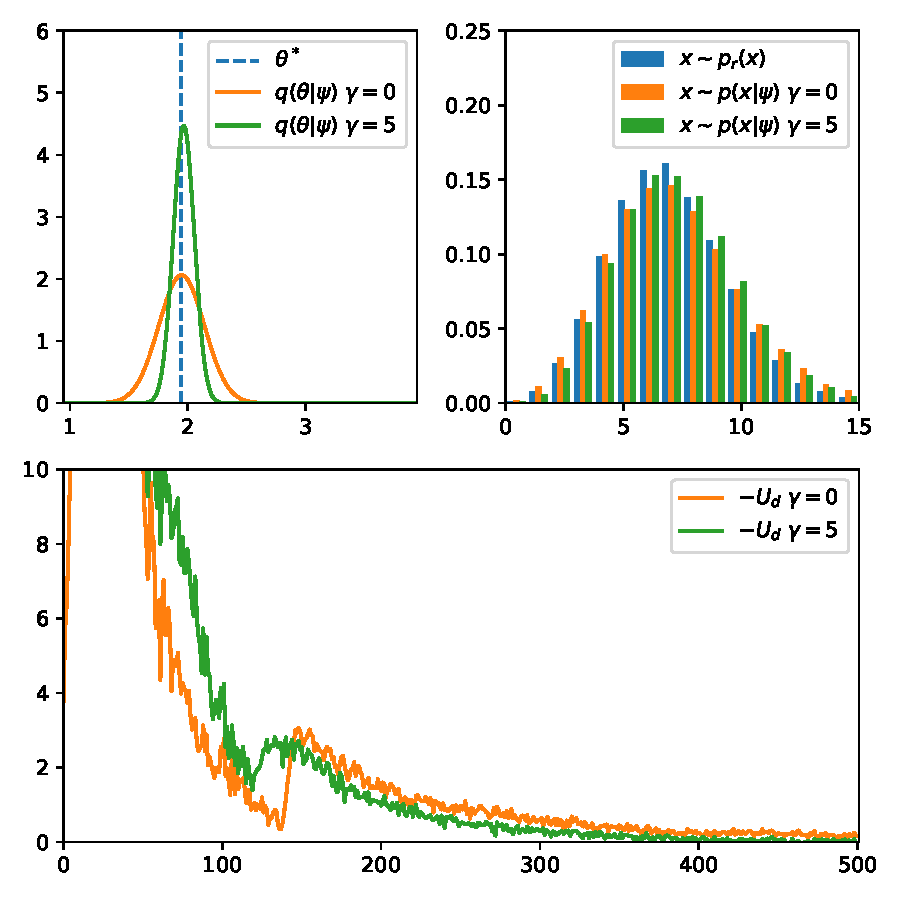
\includegraphics[width=0.48\textwidth]{figures/poisson.pdf}
\caption{Discrete Poisson model with unknown mean.
 ({\it Top left}) Proposal distributions $q(\bftheta|\bfpsi)$ after training. For both $\gamma=0$ and $\gamma=5$, the distributions correctly concentrate their density around
            the true value $\log(\lambda^*)$. Entropic regularization ($\gamma=5$) results in a tighter density.
 ({\it Top right}) Model distributions $\qxpsi$ after training. This plot shows that the resulting parametrizations of the simulator closely reproduce the true distribution.
 ({\it Bottom}) Empirical estimates of the variational upper bound $U_d$ as optimization progresses.
 }\label{fig:poisson}
\end{figure}


\subsection{Multidimensional continuous data}

As a second toy example, we consider a generator producing
5-dimensional continuous data, as originally specified in Section 4.2 of
\cite{cranmer2015approximating}.
% More specifically, we consider the following
% generative process:
% \begin{itemize}
% \item $\bfz = (z_0, z_1, z_2, z_3, z_4)$, such that \\
% $z_0 \sim {\cal N}(\mu=\alpha, \sigma=1)$,
% $z_1 \sim {\cal N}(\mu=\beta, \sigma=3)$,
% $z_2 \sim {\text{Mixture}}[\frac{1}{2}\,{\cal N}(\mu=-2, \sigma=1), \\  \frac{1}{2}\,{\cal N}(\mu=2, \sigma=0.5)]$,
% $z_3 \sim {\text{Exponential}(\lambda=3)}$, and
% $z_4 \sim {\text{Exponential}(\lambda=0.5)}$;
% \item $\mathbf{x} = R  \bfz$, where $R$ is a fixed
% semi-positive definite $5 \times 5$ matrix defining a fixed projection
% of $\bfz$ into the observed space.
% \end{itemize}
Again, AVO does not have access to the density or its gradient, only samples from the generative model.
We consider observed data generated at the nominal values $\bftheta^* = (\alpha^*=1,\beta^*=-1)$.
The simulator parameters are modeled with a factored  (mean field) Gaussian
proposal distribution $q(\bftheta|\bfpsi) = q(\alpha|\bfpsi) q(\beta|\bfpsi)$, where each component was
initialized with zero mean and unit variance.
Hyper-parameters are set to $M=64$, $n_\text{critic}=10$, $\lambda=0.1$, $\gamma=1$ and
Adam configured with a step size $\alpha=0.005$ and $\beta_1=\beta_2=0.05$.
The architecture of the critic is the same as in the previous example.

Starting with a proposal distribution $q(\bftheta|\bfpsi)$ largely spread over
the parameter space, as illustrated in the left plot of Figure~\ref{fig:multi},
AVO converges towards a proposal distribution whose density
concentrates around the nominal values $\bftheta^*$, as shown in the right plot of Figure~\ref{fig:multi}.
Overall, this example further illustrates and confirms the ability of adversarial
variational optimization for inference with multiple parameters and multidimensional
data, where reliable approximations of $p(\mathbf{x}|\bftheta)$ in a traditional
MLE setting would otherwise be difficult to construct.

\begin{figure}
\centering
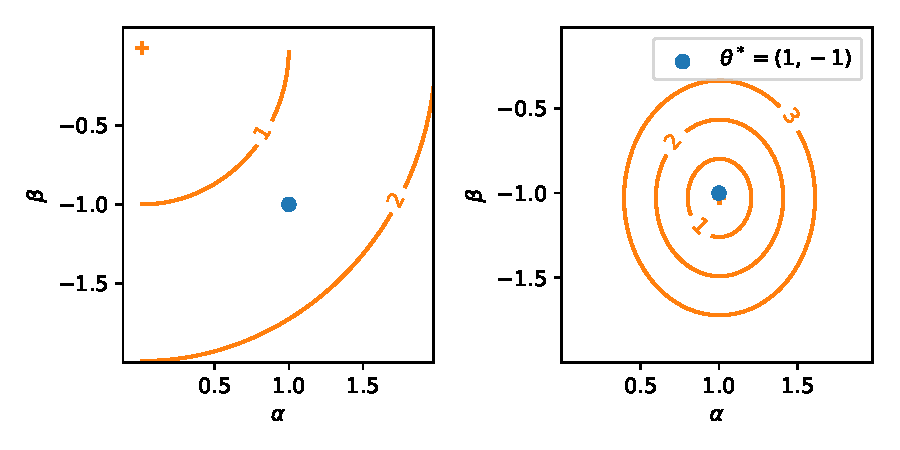
\includegraphics[width=0.48\textwidth]{figures/multi.pdf}
\caption{Multidimensional continuous data.
 ({\it Left}) Density $q(\bftheta|\bfpsi)$ at the beginning of the procedure, for a proposal distribution initialized with zero mean and unit variance.
              Contours correspond to parameters $\bftheta$ within $1$-$2$-$3$ Mahalanobis distance units from the mean of $q(\bftheta|\bfpsi)$.
 ({\it Right}) Density $q(\bftheta|\bfpsi)$ after adversarial variational optimization ($\gamma=10$).
               The proposal density correctly converges towards a distribution whose density concentrates around $\bftheta^* = (1, -1)$.
 }\label{fig:multi}
\end{figure}

% \subsection{Benchmarks}
%
% \glnote{Compare against ABC and others.}
% \glnote{Sections 6.1 and 6.4 of Bernton.}

\subsection{Electron--positron annihilation}

\begin{figure}[h]
\centering
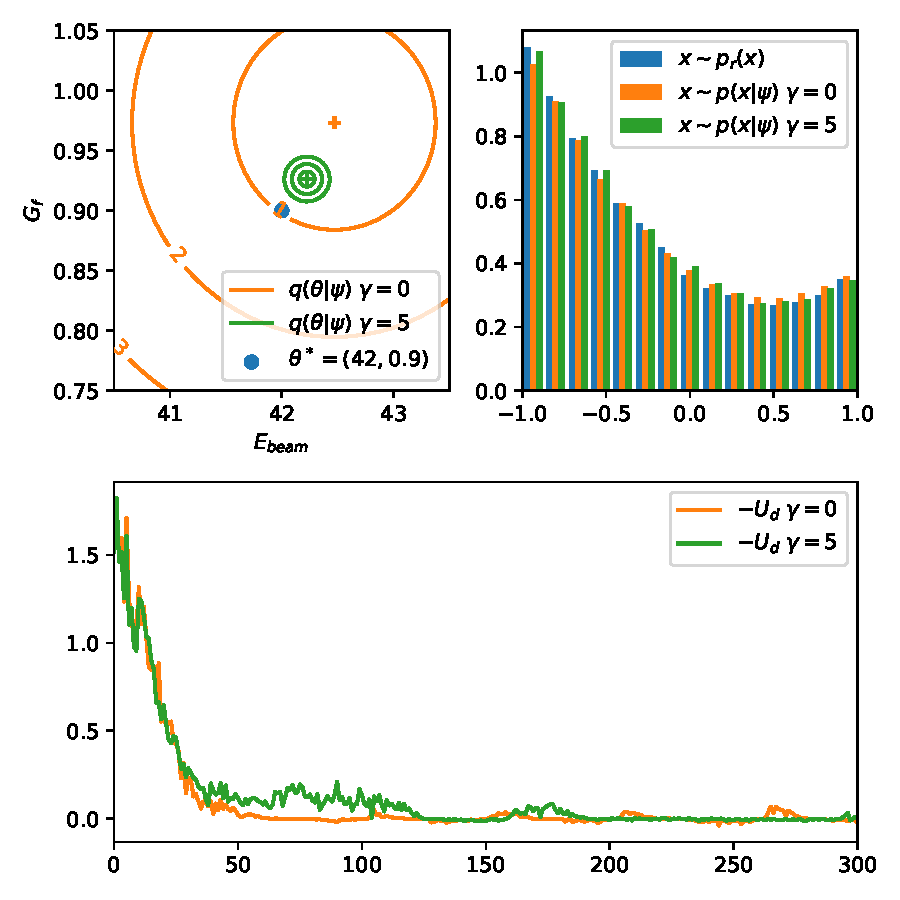
\includegraphics[width=0.48\textwidth]{figures/weinberg.pdf}
\caption{Electron--positron annihilation.
({\it Top left}) Proposal distributions $q(\bftheta|\bfpsi)$ after adversarial variational optimization.
         Contours correspond to parameters $\bftheta$ within $1$-$2$-$3$ Mahalanobis distance units from the mean of $q(\bftheta|\bfpsi)$.
         The density of the entropically regularized distribution ($\gamma=5$) is  highly concentrated, resulting in the green mass near $\bftheta^*$.
({\it Top right}) Model distributions $\qxpsi$ after training. Despite the differences between their proposal distributions, both models closely match the observed data.
({\it Bottom}) Empirical estimates of the variational upper bound $U_d$ as optimization progresses.
 }\label{fig:weinberg}
\end{figure}

As a more realistic example, we here consider a (simplified) simulator from
particle physics for electron--positron collisions resulting in muon--antimuon
pairs ($e^+e^- \rightarrow \mu^+\mu^-$). The simulator approximates the
distribution of observed measurements $\mathbf{x} = \cos(A) \in [-1,1]$, where $A$ is the
polar angle of the outgoing muon with respect  to the originally incoming
electron. Neglecting measurement uncertainty induced from the particle detectors,
this random variable is approximately distributed as
\begin{equation}\label{eq:simple_weinberg}
p(\mathbf{x}|E_\text{beam}, G_f) = \frac{1}{Z} \left[ (1 + \mathbf{x}^2) + c(E_\text{beam}, G_f) \mathbf{x} \right]
\end{equation}
where $Z$ is a known normalization constant and $c$ is an asymmetry coefficient
function. Due to the linear term in the expression, the density $p(\mathbf{x} |
E_\text{beam}, G_f)$ exhibits a so-called {\it forward-backward} asymmetry.  Its
size depends on the values of the parameters $E_\text{beam}$ (the beam energy)
and $G_f$ (the Fermi constant) through the coefficient function $c$.

A typical physics simulator for this process includes a more precise treatment of the
quantum mechanical  $e^+e^- \rightarrow \mu^+\mu^-$ scattering
using \texttt{MadGraph}~\cite{Alwall:2011uj},  ionization of matter in the
detector due to the passage of the out-going $\mu^+\mu^-$ particles using
\texttt{GEANT4}~\cite{Agostinelli:2002hh}, electronic noise and other details of the sensors
that measure the ionization signal, and the deterministic algorithms that
estimate the polar angle $A$ based on the sensor readouts. The simulation of
this process is highly non-trivial as is the space of latent variables $\mathcal{Z}$.

In this example, we consider observed data generated with the simplified generator of Eqn.~\ref{eq:simple_weinberg}
using $\bftheta^* = (E_\text{beam}^*=42, G_f^*=0.9)$. The simulator parameters are modeled with a
factored (mean field) Gaussian proposal distribution $q(\bftheta|\bfpsi) = q(E_\text{beam}|\bfpsi)
q(G_f|\bfpsi)$, where each component is respectively initialized with mean $45$
and $1$ and variance $1$ and $0.01$. Hyper-parameters are set to $M=64$,
$n_\text{critic}=100$, $\lambda=0.0025$ and Adam configured with $\alpha=0.01$,
$\beta_1=0.9$ and $\beta_2=0.999$. As with the first example, we compare
entropy penalties $\gamma=0$ and $\gamma=5$. \glnote{Double check}

The top left plot in Figure~\ref{fig:weinberg} illustrates the resulting
proposal distributions $q(\bftheta|\bfpsi)$ for $\gamma=0$ and $\gamma=5$ after
AVO. We see that the distributions both arrive
in the neighborhood of $\bftheta^*$, with a density  more highly concentrated for
$\gamma=5$ than for $\gamma=0$.  Despite these differences and the relative
distance with $\bftheta^*$, both models closely match the observed data, as shown
in the top right plot of  Figure~\ref{fig:weinberg}, with again slightly better
results when using entropic regularization. This suggests either a relatively flat
landscape around $\bftheta^*$ or that the observed data can in this case also be
reproduced with the  predictive distribution $\qxpsi$.
Finally, the bottom plot of Figure~\ref{fig:weinberg} shows that for both
$\gamma=0$ and $\gamma=5$ the variational upper bound $-U_d$ fall
towards $0$, which indicates  convergence towards a distribution that the critic
cannot distinguish from the true distribution.


% ==============================================================================

\section{Related work}

This work sits at the intersection of several lines of research related to
likelihood-free inference, approximate Bayesian computation (ABC),
implicit generative models, and variational inference.
Viewed from the literature around implicit generative models based on neural networks,
the proposed method can be considered as a direct adaptation of
generative adversarial networks~\cite{goodfellow2014generative,2017arXiv170104862A} to
non-differentiable simulators using variational optimization~\cite{2012arXiv1212.4507S}.

From the point of view of likelihood-free inference, where  non-differentiable
simulators are the norm, our contributions are threefold. First is the process
of lifting the expectation with respect to the non-differentiable simulator
$\mathbb{E}_{\tilde{\bfx} \sim p(\bfx | \bftheta)}$ to a differentiable
expectation with respect to the variational program $\mathbb{E}_{\tilde{\bfx}
\sim q(\bfx | \bfpsi)}$. Secondly, is the introduction of a novel form of
variational inference that works in a likelihood-free setting. Thirdly, the
AVO algorithm can be viewed as a form of empirical Bayes where the prior is
optimized based on the data.

Perhaps the closest to our work is~\cite{bernton2017inference}, which uses the
Wasserstein distance both to find point estimates $\bftheta^*$ and as a part of
a rejection sampler in an ABC-like setup (as opposed to variational inference).
They emphasize that this approach allows one to eliminate the summary statistics
typically used in ABC and calculate the Wasserstein distance explicitly, without
making use of the Kantorovich-Rubinstein duality and of a critic $d$. For high-dimensional
data, they note that this is computationally expensive and introduce an
approximation based on projection of the data onto Hilbert space-filling curves.
Their Remark 5.1 points out that~\cite{montavon2016wasserstein} proposed an
approximation of the gradient of an entropy-regularized Wasserstein distance,
which uses a similar duality. They note that ``unfortunately, it is not
applicable in the setting of purely generative models, as it involves point-wise
evaluations of the derivative of the log-likelihood.'' Thus, our contribution is
to provide gradients of an approximate MWE by taking expectations with the
variational program $q(\bfx | \bfpsi)$. This paired with the critic
Kantorovich-Rubinstein dual formulation of the Wasserstein distance
allows us to work in high dimensions without summary statistics and to
optimize $\bfpsi$ with stochastic gradient descent. Additionally,
our procedure avoids the inefficiencies of
their Wasserstein rejection sampler incurred from using the ABC-likelihood.
In the case of small $N$, we note however that fast algorithms for calculating the exact (entropically regularized) Wasserstein distance on
empirical distributions~\cite{cuturi2013sinkhorn, genevay2016stochastic, montavon2016wasserstein}
are alternatives to adversarial learning that are worth considering.

More generally, likelihood-free
inference is intimately tied to a class of algorithms that can be framed as
density estimation-by-comparison, as reviewed in \cite{2016arXiv161003483M}. In most cases, these
inference algorithms are formulated as an iterative two-step process where the
model distribution is first compared to the true data distribution and then
updated to make it more comparable to the latter. Relevant work in this
direction includes those that rely on a classifier to estimate the discrepancy between the observed data and the model distributions
\cite{gutmann2012noise,cranmer2015approximating,cranmer2016experiments,2016arXiv161110242D,gutmann2017likelihood,rosca2017variational}.
Also of direct relevance in the likelihood-free setup, Hamiltonian ABC~\cite{meeds2015hamiltonian}
estimate gradients with respect
to $\bftheta$ through finite differences from multiple forward passes of the
simulator with variance reduction strategies based on controlling the source of
randomness used for the latent variable $\bfz$.

Likewise, AVO closely relates to recent extensions of GANs, such as
Adversarial Learned Inference (ALI)~\cite{dumoulin2016adversarially},
Bidirectional GANs (BiGANs)~\cite{donahue2016adversarial},
$\alpha$-GAN~\cite{rosca2017variational}, Adversarial Variational Bayes
(AVB)~\cite{DBLP:journals/corr/MeschederNG17}, and the \texttt{PC-Adv}
algorithm of  \cite{2017arXiv170208235H}, which
add an inference network to the generative model.  Each of these assume a
tractable density $p(\bfx|\bftheta)$ that is differentiable with respect to
$\bftheta$, which is  not satisfied in the likelihood-free setting. Our lifting
of the non-differentiable simulator $p(\bfx|\bftheta)$ to the variational
program $q(\bfx | \bfpsi)$ provides the ability to differentiate expectations
with respect to $\bfpsi$ as in Eqn~\ref{eqn:approx-grad}; however, the density
$q(\bfx | \bfpsi)$ is still intractable. Moreover, we do not attempt to define a
recognition model  $q(\bfz, \bftheta|\bfpsi)$ as the latent space $\mathcal{Z}$
of many real-world simulators is complicated and not amenable to a neural
recognition model.

This work has also many connections to work on variational inference, in which
the goal is to optimize the recognition model $q(\bfz, \bftheta|\bfpsi)$ so that
it is close to the true posterior $p(\bfz, \bftheta |\mathbf{x})$. There have
been efforts to extend variational inference to intractable likelihoods;
however, many require restrictive assumptions.  In \cite{tran2017variational},
the authors consider Variational Bayes with an Intractable Likelihood (VBIL). In
that approach ``the only requirement is that the intractable likelihood can be
estimated unbiasedly.'' In the case of simulators, they propose to use the
ABC-likelihood with an $\epsilon$-kernel. The ABC likelihood is only unbiased as
$\epsilon \to 0$,   thus this method inherits the drawbacks of the
ABC-likelihood including the choice of summary statistics and the inefficiency
in evaluating the ABC likelihood for high-dimensional data and small $\epsilon$.
More recently, \cite{2017arXiv170208896T} adapted variational inference to
hierarchical implicit models defined on simulators. In this work, the authors
step around the intractable likelihoods by reformulating the optimization of the
ELBO in terms of a neural and differentiable approximation $r$ of the log-likelihood
ratio $\log \tfrac{p}{q}$, thereby effectively using the same core principle as used
in GANs~\cite{2016arXiv161003483M}.

Lastly, we make a connection to Operator Variational Inference (OPVI)~\cite{2016arXiv161009033R},
which is a generalization of variational inference formulated as the following optimization problem:
\begin{eqnarray}
\bflambda^* = \inf_\bflambda \sup_\bfphi \mathbb{E}_{ \bfz \sim q( \bfz | \bflambda)} [ (O^{p,q} f_\bfphi) ] \, .
\end{eqnarray}
In traditional VI with the KL distance, this corresponds to $(O^{p,q} f)(\bfz) = \log q(\bfz) - \log p(\bfz|\bfx) \, \forall f \in \mathcal{F}$.
AVO can be cast into a similar form with expectations over $\bfx$ instead of $\bfz$ and
\begin{eqnarray} \label{eq:opvi_avo}
\bfpsi^* &=& \inf_\bfpsi \sup_\bfphi \mathbb{E}_{ \bfx \sim q( \bfx | \bfpsi)} [ (O^{p_r,q_\bfpsi} d_\bfphi) ] \\
\label{eq:opvi_avo2} &=&  \inf_\bfpsi \sup_\bfphi \mathbb{E}_{\bfx\sim p_r(\bfx)}[d(\bfx; \bfphi)] - \mathbb{E}_{\bfx \sim q(\bfx|\bfpsi)}[d(\bfx; \bfphi)] \nonumber \, .
\end{eqnarray}
Rewriting Eqn.~\ref{eq:opvi_avo} as above is possible through importance sampling,
corresponding to an implicit form of the operator
\begin{equation}
(O^{p_r,q_\bfpsi} d_\bfphi)(\bfx) = \left( \frac{p_r(\bfx)}{q(\bfx|\bfpsi)}  -1 \right) d(\bfx; \bfphi) \, ,
\end{equation}
which reinforces the link to density ratio estimation and inference with implicit models.


% ==============================================================================

\section{Summary}

In this note, we develop a likelihood-free inference algorithm for
non-differentiable, implicit generative models. The algorithm combines
adversarial training  with variational optimization to minimize variational
upper bounds  on the otherwise non-differentiable adversarial objectives. The
AVO algorithm enables empirical Bayes through variational inference in the
likelihood-free setting. This approach does not incur the inefficiencies of an
ABC-like rejection sampler. When the model is well-specified, the AVO algorithm
provides point estimates for
the generative model, which asymptotically corresponds to the data generating
parameters. The algorithm works on continuous or discrete data.

Preliminary results on toy problems with discrete and continuous data validate
the proposed method. While the obtained results are encouraging, the complete
validation of the method remains to be carried out in real conditions on a full
fledged scientific simulator -- which we plan to achieve for a next version of
this work \glnote{to update}. In terms of method, several components need further investigation.
First, we need to better study the interplay between the entropic regularization and the
adversarial objectives. Second, we should better understand the dynamics of the
optimization procedure, in particular when combined with momentum-based
optimizers like Adam. Third, we need to consider whether less noisy estimates of
the gradients $\nabla_\bfpsi U_g$ can be computed.


% ==============================================================================

% \section*{Acknowledgements}

% We would like to thank Lukas Heinrich for helpful comments regarding
% the electron--positron annihilation simulation. We would also like to thank
% Rajesh Ranganath and Dustin Tran for enlightening discussions and feedback.
% GL and KL are both supported through NSF ACI-1450310, additionally KC is
% supported through PHY-1505463 and PHY-1205376.

\bibliography{bibliography.bib}
\bibliographystyle{icml2018}

% ==============================================================================

% \appendix
%
% \section{Further experiments}


\end{document}
